\section{Vista de casos de uso}
\label{sec:casos-de-uso}

Esta vista presenta los objetivos del cliente y las interacciones externas
del sistema. Aporta los casos y escenarios de la vista $+1$ del modelo $4+1$.
Los cinco casos corresponden a las consultas Q1--Q5 del DAG y comparten los
artículos enviados en una ejecución. Su representación por separado identifica
los resultados esperados; no prescribe cinco conexiones ni cinco envíos del
dataset.

\subsection{Actores y alcance}
\label{subsec:actores-casos-uso}

El \textbf{Cliente} es la aplicación que dispone del dataset, envía los
artículos en inglés y francés y recibe los resultados y el estado de la
ejecución. Es el actor principal de los cinco casos. La dirección de su
Gateway está configurada previamente, como se describe en la
sección~\ref{subsec:despliegue}.

\textbf{Wikimedia} es el actor externo de apoyo de CU2: proporciona los
metadatos y el contenido de las imágenes referenciadas por los artículos.
El límite del sistema incluye Gateway, ResultCollector, los workers y
RabbitMQ; estos componentes internos se desarrollan en las otras vistas.
Las asociaciones de la figura~\ref{fig:casos-de-uso} indican participación,
sin representar un orden de ejecución ni canales de comunicación internos.

\begin{figure}[htbp]
    \centering
    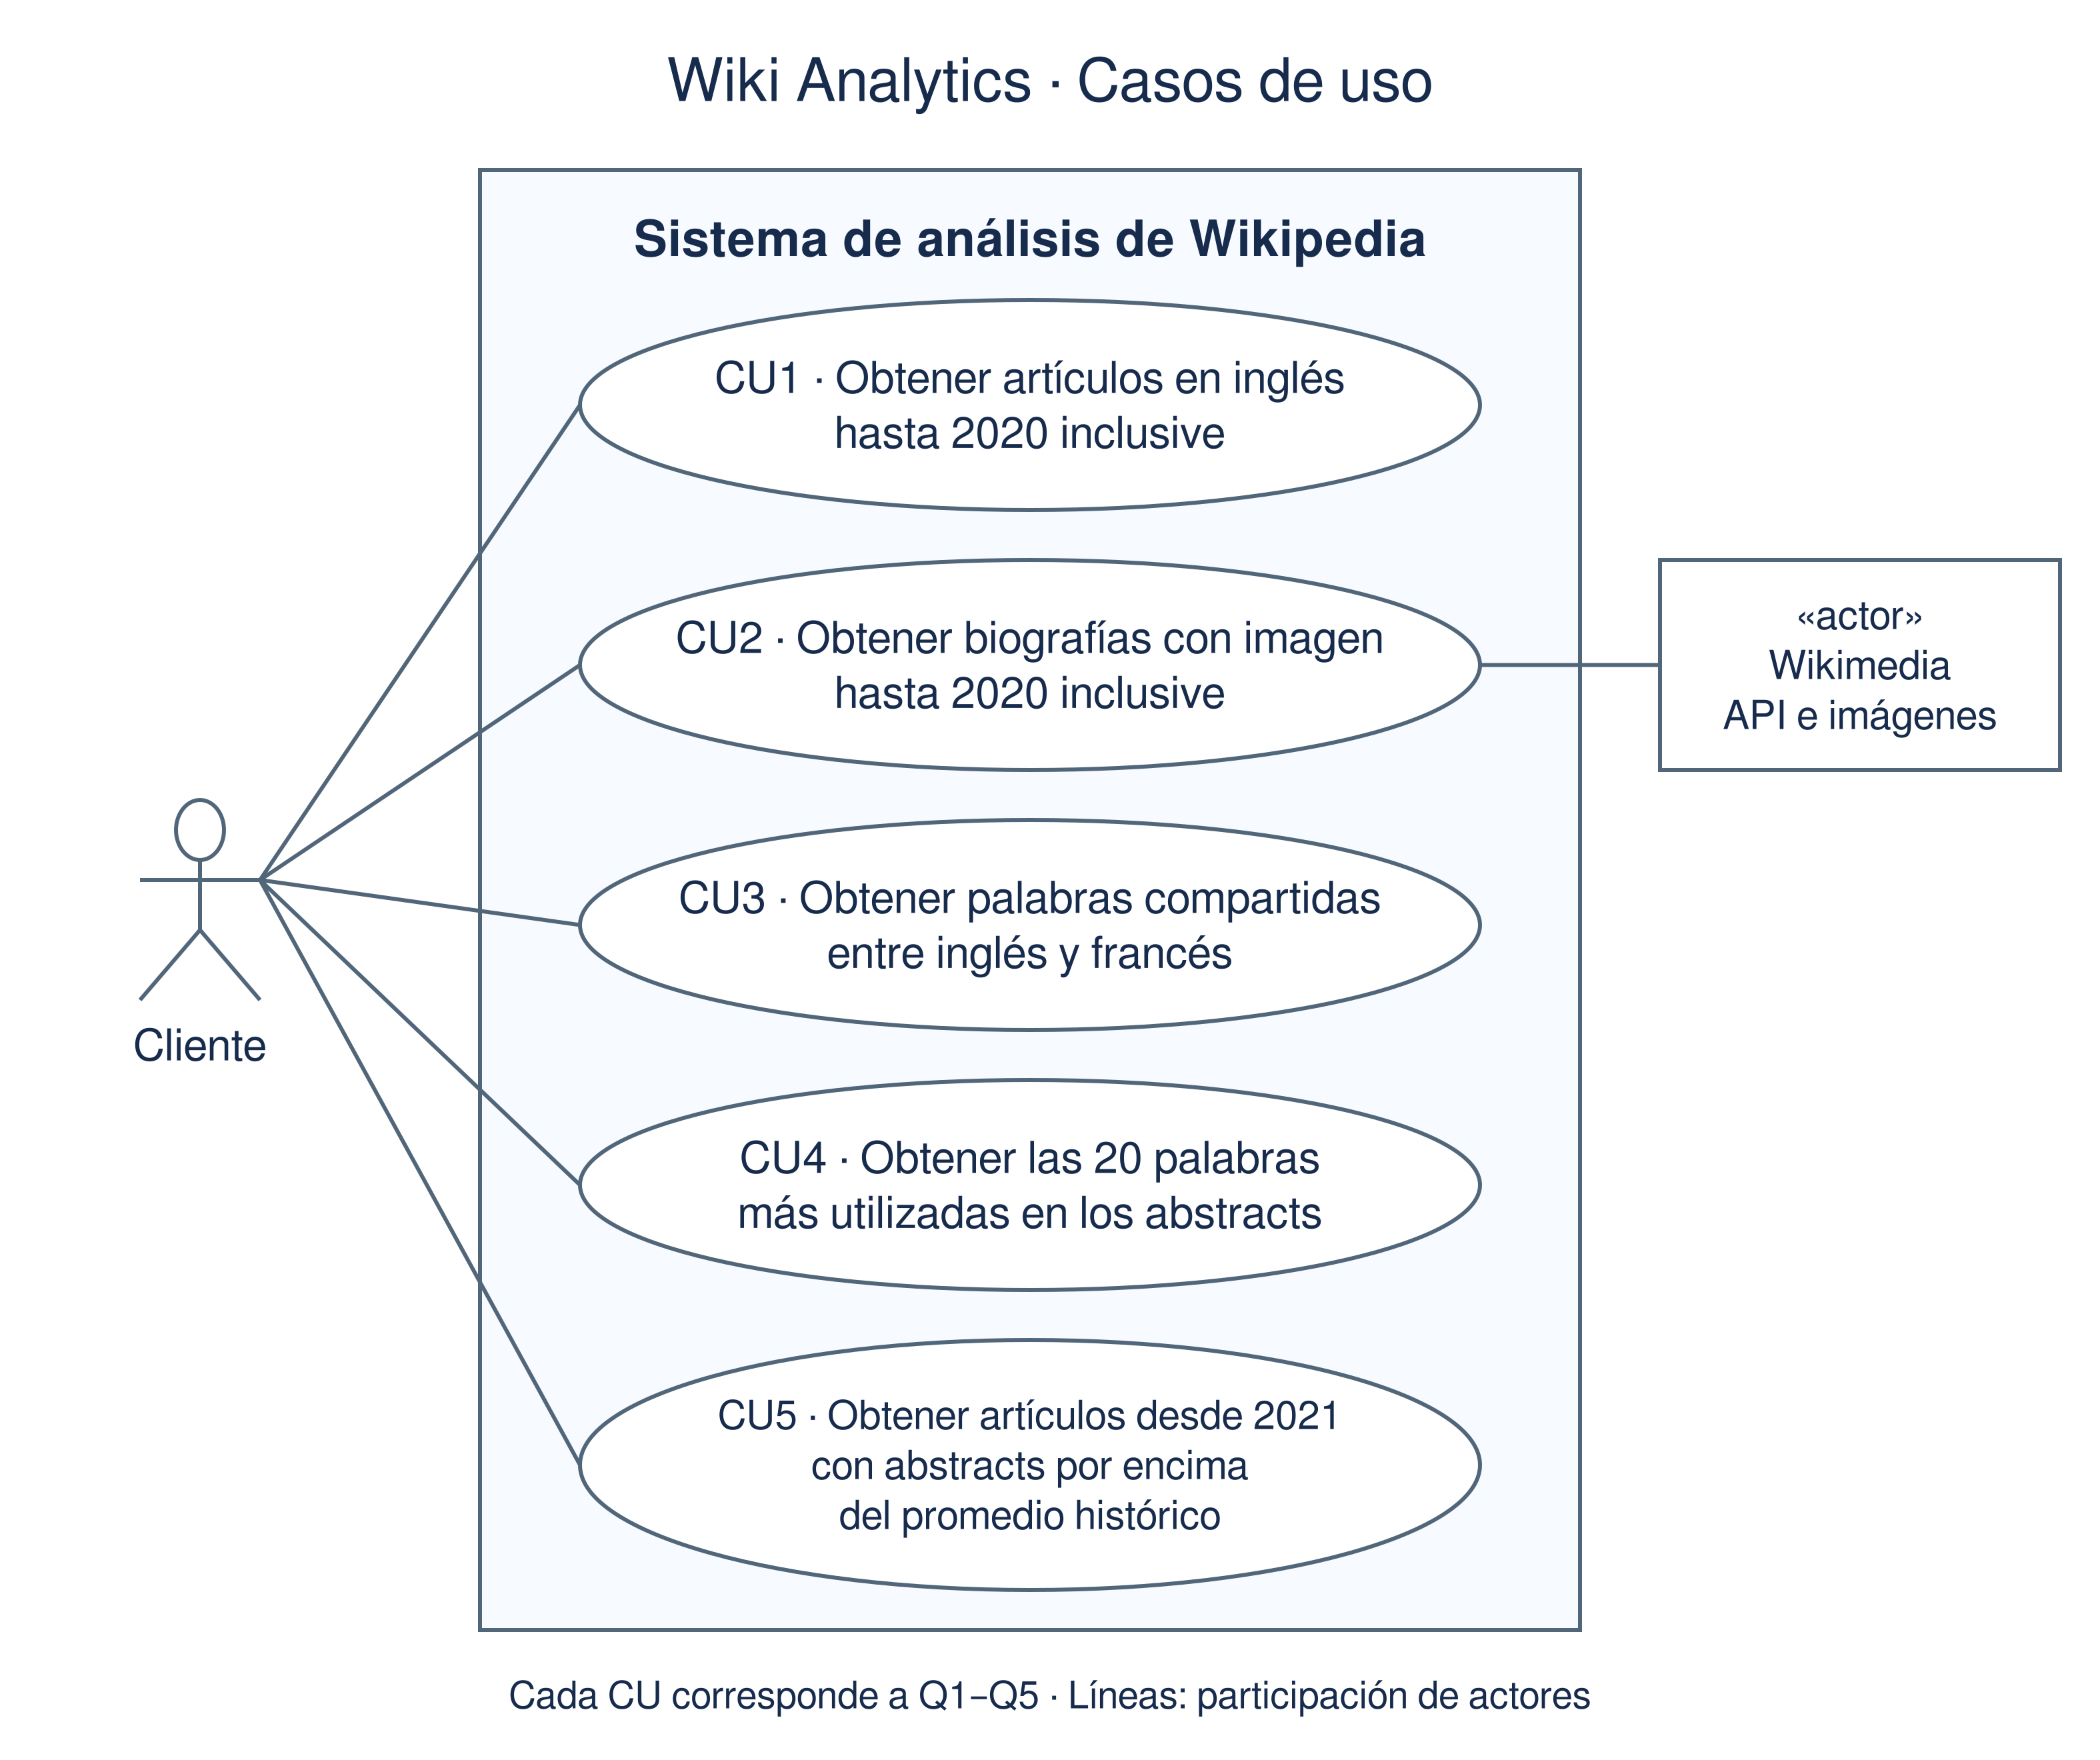
\includegraphics[width=\textwidth,height=0.70\textheight,keepaspectratio]{img/diagrama_de_casos_de_uso.png}
    \caption{Casos de uso del sistema de análisis de Wikipedia. El Cliente
    obtiene los resultados de Q1--Q5; Wikimedia participa en la obtención
    de imágenes para Q2.}
    \label{fig:casos-de-uso}
\end{figure}

\subsection{Resultados de los casos de uso}
\label{subsec:resultados-casos-uso}

Los cortes temporales se aplican a la fecha de última modificación
(\texttt{date\_modified}). Cada caso opera sobre los datos de su ejecución,
sin combinar los artículos de clientes diferentes.

\begin{description}
    \item[CU1 (Q1).] \textbf{Obtener artículos en inglés hasta 2020 inclusive.}
    El cliente obtiene la URL y la fecha de modificación de los artículos
    en inglés que cumplen el corte temporal.

    \item[CU2 (Q2).] \textbf{Obtener biografías con imagen hasta 2020 inclusive.}
    El cliente obtiene nombre, URL del artículo y bytes de imagen para los
    artículos que cumplen el corte temporal y contienen una sección denominada
    \texttt{biography} o \texttt{biographie}, comparada en minúsculas.
    El sistema obtiene las imágenes de Wikimedia cuando existe una referencia.
    La salida acordada sigue el enunciado: incluye la URL del artículo en lugar
    de la fecha propuesta en V1.

    \item[CU3 (Q3).] \textbf{Obtener palabras compartidas entre inglés y francés.}
    El cliente obtiene las palabras únicas presentes en al menos un abstract
    en inglés y al menos uno en francés. Se utiliza el vocabulario normalizado
    de los abstracts, excluyendo stopwords y tokens numéricos.

    \item[CU4 (Q4).] \textbf{Obtener las 20 palabras más utilizadas en los abstracts.}
    El cliente obtiene hasta 20 pares (palabra, cantidad), correspondientes
    a las palabras con mayor conteo entre todos los abstracts de la ejecución.
    Se excluyen stopwords y cada palabra aporta una sola unidad por abstract.

    \item[CU5 (Q5).] \textbf{Obtener artículos desde 2021 con abstracts por encima del
    promedio histórico.}
    El cliente obtiene la URL y el conteo de palabras de los artículos desde
    2021 cuyo abstract supera estrictamente el promedio de los abstracts de
    artículos hasta 2020 inclusive. Al igual que en Q4, se excluyen stopwords
    y se cuenta cada palabra distinta una sola vez por abstract.
\end{description}

\subsection{Escenario común de ejecución}
\label{subsec:escenario-comun}

La precondición es que el cliente disponga del dataset y pueda establecer
la conexión con el Gateway configurado. El escenario satisfactorio comprende:
\begin{enumerate}
    \item El cliente inicia una ejecución y envía incrementalmente sus
    artículos al sistema.
    \item El sistema procesa las cinco consultas con estado aislado para esa
    ejecución. El cliente recibe resultados mientras continúa enviando datos;
    Q1, Q2 y Q3 permiten entregas parciales.
    \item El cliente indica el fin de la entrada. El sistema completa el
    procesamiento pendiente; Q4 y Q5 entregan resultados después de procesar
    toda la entrada, aunque su salida pueda transmitirse en lotes.
    \item El cliente recibe la finalización de cada consulta y de la ejecución.
    Una finalización exitosa indica que se entregaron todos los resultados
    correspondientes, incluyendo consultas sin coincidencias.
\end{enumerate}

\paragraph{Variantes y terminaciones no exitosas.}
En CU2, una referencia de imagen ausente se informa explícitamente. Si existe
una referencia pero su descarga falla definitivamente, Q2 se informa como
fallida y los resultados parciales no se presentan como una respuesta completa.
En CU5, si no hay abstracts históricos computables, se devuelve un resultado
vacío con el estado \emph{sin base histórica}.

Una caída abrupta aborta las ejecuciones afectadas. Un nuevo intento utiliza
otra identidad de ejecución y retransmite toda la entrada; el cliente no
acumula los resultados del intento fallido. Ante SIGTERM, el sistema coordina
la finalización de las ejecuciones activas o notifica una cancelación explícita,
sin anunciar éxito para una ejecución incompleta. Las condiciones operativas
se detallan en la vista física y la gestión de estado en la
sección~\ref{subsec:estado-recursos}.

